
\documentclass[preprint,12pt]{elsarticle}

\usepackage[spanish]{babel}
\usepackage{amssymb}
\usepackage{graphicx}
\usepackage{lineno}
\usepackage[utf8]{inputenc}
\usepackage{url}
\usepackage{natbib}

\begin{document}
	
	\begin{frontmatter}

		\title{\huge  SISTEMA DE ATENCIÓN AL CLIENTE - PANNTONY}
		
		\author{Estrella Palacios, Katherine Lizbeth      (2015050948)}		
		\author{Robles Flores, Anthony Richard	(2016056192)}
		\author{Sandoval Blas, Jesus Enrique           	(2016054467)}
		\author{Atahuachi Rivera, Gabriela            	(2015053235)}
		
		\address{Tacna, Perú}
		
		\begin{abstract}
Customer service is defined as a service that the same company provides to the client, in order to interact with it and that can evaluate the services that the organization offers as the product that is within the factors is quality, taste , freshness, presentation and variety; In this way the organization will be able to know if it reached its real purpose that is to satisfy the needs of the client. In this project an application will be developed for the company La Favorita Alimentos S.A.C. located in the city of Tacna and distributor of the Panttony brand, whose objective will be to provide the company with a tool for feedback and qualification of customer service.
		\end{abstract}
\end{frontmatter}

\section{Resumen}
La atención al cliente se define como un servicio que la misma empresa otorga al cliente, con la finalidad de interrelacionar con él y que pueda evaluar los servicios que la organización ofrece como el producto que dentro de los factores se encuentran la calidad , el sabor , la frescura , la presentación y su variedad; de esta  manera la organización podrá saber si llego a su finalidad real que es satisfacer las necesidades del cliente. En el presente proyecto se desarrollara un aplicativo para la empresa La Favorita Alimentos S.A.C. ubicada en la ciudad de Tacna y distribuidora de la marca Panttony, cuyo objetivo será brindar a la empresa una herramienta de retroalimentación y calificación de la atención al cliente.

\section{Introducción}
%%https://www.crecenegocios.com/que-es-el-servicio-al-cliente-y-cual-es-su-importancia/
En Perú la competencia es cada vez mayor y los productos ofertados en el mercado son cada vez más variados, los consumidores se vuelven cada vez más exigentes. Ellos ya no solo buscan calidad y buenos precios, sino también un buen servicio al cliente.
El servicio al cliente es el servicio o atención que una empresa o negocio brinda a sus clientes al momento de atender sus consultas, pedidos o reclamos, venderle un producto o entregarle el mismo.\\
\\Cuando un cliente encuentra el producto que buscaba, y además recibe un buen servicio al cliente, queda satisfecho y esa satisfacción hace regrese y vuelva a comprarnos, y que muy probablemente nos recomiende con otros consumidores.
Pero por otro lado, si un cliente, haya encontrado o no el producto que buscaba, recibe una mala atención, no solo dejará de visitarnos, sino que muy probablemente también hablará mal de nosotros y contará la experiencia negativa que tuvo a un promedio de entre 9 a 20 personas dependiendo de su grado de indignación.
Si a ello le sumamos el hecho de que la competencia cada vez es mayor y los productos ofertados en el mercado se equiparan cada vez más en calidad y en precio, es posible afirmar que hoy en día es fundamental brindar un buen servicio al cliente si queremos mantenernos competitivos en el mercado.\\
\\Debemos evitar que el cliente sea mal atendido, y así que deje de visitarnos o pueda llegar a hablar mal de nosotros, y más bien procurar que reciba un buen servicio al cliente, y así lograr su fidelización, tener buenas posibilidades de que nos recomiende con otros consumidores, y poder diferenciarnos o destacar ante los demás competidores.\\
\\En la empresa La Favorita Alimentos S.A.C. ubicada en la ciudad de Tacna y distribuidora de la marca Panttony, existe una problemática el cual es que carece de una herramienta que permita al cliente poder evaluar sus diferentes servicios donde podemos englobar PRODUCTO (calidad , Sabor, Frescura, presentación, variedad) , SERVICIO (Rapidez, cordialidad, presentación del personal) y LOCAL (Ambiente y decoración , limpieza) , por lo tanto la empresa busca mejorar cada vez mas sus servicios por eso es de vital importancia esta herramienta y ofrecerlas a sus clientes como fin de ser calificadas y ser subsanadas en sus proceso de cada fase .


\section{Título}
SISTEMA DE ATENCION AL CLIENTE - PANNTONY

\section{Autores}
\begin{itemize}
	\item Estrella Palacios, Katherine Lizbeth
	\item Robles Flores, Anthony Richard
	\item Sandoval Blas, Jesus Enrique
	\item Atahuachi Rivera, Gabriela    
\end{itemize}

\section{Planteamiento del problema}
	\subsection{Problema }	
		La organización buscar mejorar cada vez más sus diferentes módulos de servicios como los productos, servicios, atención y local.
		Existe una problemática el cual es que en el transcurso del día se acerca a la organización una cantidad numerosa de clientes que su finalidad es solo poder consumir o poder utilizar los servicios o productos que ofrecen.
		La empresa busca mejorar cada vez más tomando en cuenta las diferentes competencias existentes en el mercado, para lo cual carece de una herramienta o plataforma que permita calificar sus diferentes módulos de servicios.

	\subsection{Justificación }	
		Al ya haber mencionado la problemática existente en la de la organización, se analizo cuidadosamente llegando  a la conclusión de poder ofrecer una sistema que permita al cliente en cada uno de sus consumos de los diferentes servicios puedan estos calificar de 			misma forma poder guardar en la base de datos las propuestas, quejas, sugerencias de los clientes hacia la organización.
	\subsection{Alcance }
		La finalidad de esta herramienta a crear será poder calificar todos los módulos de servicios que la organización provee a sus clientes, de tal manera con la acumulación de registros , la organización podrá mejorar , omitir , actualizar con el único fin de satisfacer las 			necesidades del cliente.
		Puesto que poder calificar podría ser algo estresante por parte del cliente , la misma herramienta creará un randon donde este actor podrá ser premiado por su información aportada para la empresa.


\section{Objetivos}
	\subsection{General }	
		Implementar un Sistema de Calificaciones de Atención al Cliente utilizando la herramienta NetBeans y para su conexión a base de datos la herramienta SQL Server.
	\subsection{Específico }	

\begin{itemize}
	\item Diseñar una base de datos
	\item Aplicar el paradigma  de la programación y consultas como herencia, conexiones y las variaciones de las consultas en SQL Server.
\end{itemize}


\section{Referentes Teóricos}
\subsection{Cliente}
Un cliente, desde el punto de vista de la economía, es una persona que utiliza o adquiere, de manera frecuente u ocasional, los servicios o productos que pone a su disposición un profesional, un comercio o una empresa.
\subsection{Organización}
Es un sistema diseñado para alcanzar ciertas metas y objetivos. Estos sistemas pueden, a su vez, estar conformados por otros subsistemas relacionados que cumplen funciones específicas.
\subsection{Atención al cliente}
Es aquel servicio que prestan y proporcionan las empresas de servicios o que comercializan productos, entre otras, a sus clientes para comunicarse directamente con ellos.
\subsection{Calificación}
Es una valoración personal que realiza una persona al puntuar de acuerdo a una escala de valoración gradual que puede ir de 0 a 10 un objeto determinado.
\subsection{Base de datos}
Conjunto de información perteneciente a un mismo contexto, ordenada de modo sistemático para su posterior recuperación, análisis o transmisión.
\subsection{Metodología XP}
Una metodología de desarrollo que pertenece a las conocidas como metodologías ágiles (otras son Scrum, Kanban…), cuyo objetivo es el desarrollo y gestión de proyectos con eficacia, flexibilidad y control.


\section{Desarrollo de la propuesta}
	\subsection{Tecnología de información }	
		AQUI VA EL TEXTO
	\subsection{Metodología, técnicas usadas }	
		AQUI VA EL TEXTO

\section{Cronograma}
\begin{figure}[htb]
	\begin{center}
		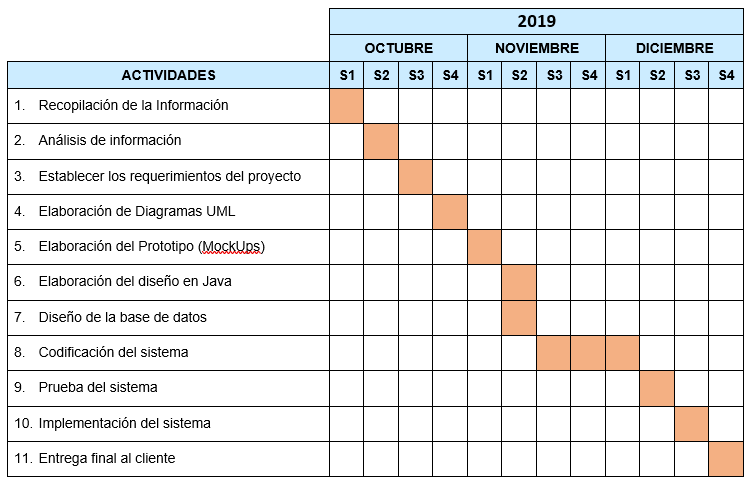
\includegraphics[width=12cm]{./IMAGENES/cronograma} 
	\end{center}
\end{figure}

\subsection{\textbf{Recursos Humanos}}
\begin{itemize}
	\item Estrella Palacios, Katherine Lizbeth (Programador / Analista)
	\item Robles Flores, Anthony Richard (Programador / Tester)
	\item Sandoval Blas, Jesus Enrique (Programador / Analista)
	\item Atahuachi Rivera, Gabriela  (Diseñadora / Tester)
\end{itemize}

\subsection{\textbf{Recursos Materiales y Servicios}}
\begin{itemize}
	\item Laptop (3)
	\item Impresora
	\item USB
	\item Impresiòn
	\item Internet
\end{itemize}
	
\section{Presupuesto (Beneficio / Costo, VAN)}
AQUI VA EL TEXTO

\section{Conclusiones y Recomendaciones }
AQUI VA EL TEXTO
(comentar dificultades y retos en el desarrollo del trabajo)



	
	\newpage
	


	

\end{document}

